\section{VoIP Standards}

Contrary to common belief VoIP is not a single protocol or protocol stack but a collection of technologies that maybe be assembled together to provide voice-like-data over the IP protocol. Simpler VoIP implementations concern themselves with the session and presentation layers of the OSI seven layer model, as illustrated. But when scaling this technology across enterprise or internet sized systems many deeper grained issues begin to appear such as fault tolerance, security, latency, mobility and quality of service.
\begin{center}
	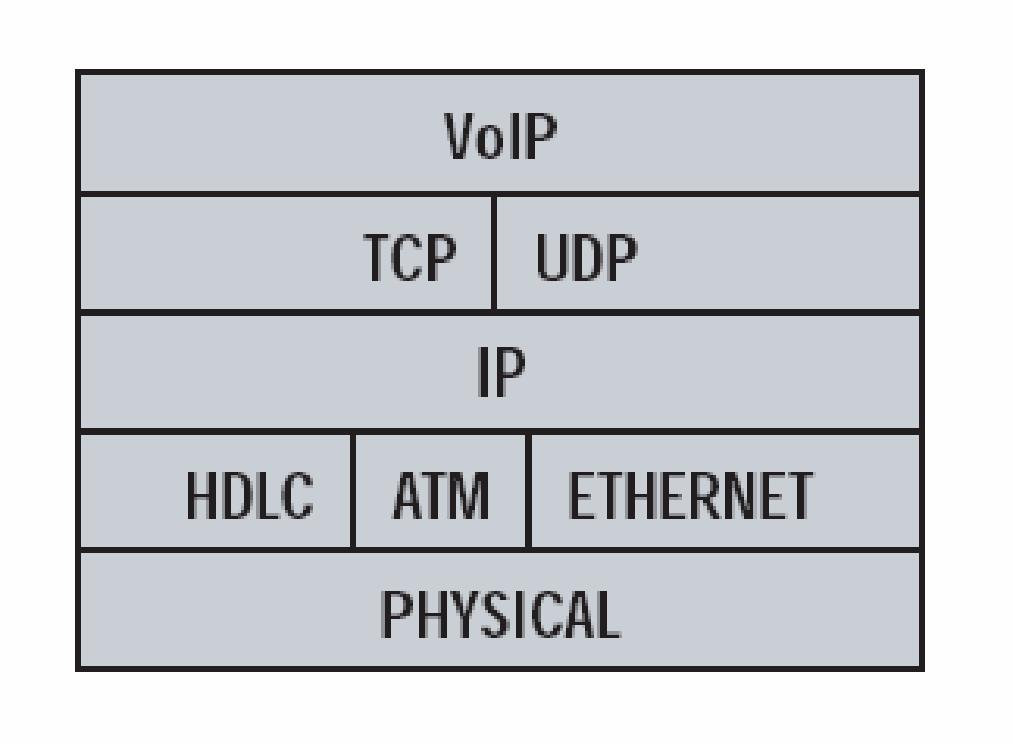
\includegraphics[width=3in]{images/simple_voip_protocol.jpg}
\end{center}

\subsection{H.323 - Packet-based multimedia communications systems}
A standard defined by the International Telecommunication Union (ITU) and was initially published in 1996\cite{website:itu_h323} the same month the SIP draft was published and was the first standards based VoIP stack\cite{website:packetizer_h323}. This standard encapsulates a number of ITU-T and IETF protocols used in the transmission of voice, video and data over a packet switched network.

The standard consists of a number of classes of components, below is a breakdown and description of these elements:

\begin{description}
\item[Terminals*] Voice and video handsets, high-definition videoconferencing systems, voicemail systems, softphones.
\item[Multipoint Control Units* (MCUs)] Responsible for managing multi-point conferences (two or more endpoints involved in  a conference).
\item[Gateways*] Interfaces to other networks e.g. PSTN, H.320 (VoIP using ISDN) or other H.323 networks (proxy).
\item[Gatekeeper] An optional component which manages admission control and address resolution and can be used to implement features such as follow-me/find-me or forward on busy.
\item[Border Elements and Peer Elements] Exchange addressing information and participate in authorisation across administrative domains. Peer elements are used to aggregate and reduce the volume of routing information exchanged across domains.
\end{description} 
*often referred to as endpoints

While all of the elements described above are not required, at minimum two terminals are required to facilitate communication between two people and in most deployments a gatekeeper is deployed to facilitate address resolution among other functions.

H.323 is described as a ‘framework’ document which defines how various protocols fit together. Common implementations of this standard may employ twelve or more protocols in to perform basic VoIP functionality. The standard covers all aspects of communication from T.120 for data conferencing to T.38 for fax transmission and from H.235 defining security to H.225.0 defining call signaling between endpoints.

From this brief overview of the standard it is quite clear to see that H.323 is a robust and complex standard defined by the telecommunications industry for the telecommunications industry. From its inception has been positioned as a ‘next generation’ to the POTS network offering voice, video, data, conferencing, roaming and other features naively while maintaining compatibility with legacy systems by way of support for PSTN numbering for example.

One criticism of this standard is its complexity due to its rigid specification for areas of the standard, which has slowed the deployment of these H.323 networks.

\subsection{SIP - Session Initiation Protocol}
Positioned as an alternative standard, the initial SIP draft document was published during the same period as the first revision of the H.323 standard in 1996. The SIP signaling protocol is published by a working group of the IETF (Internet Engineering Task Force), and due to this affiliation the standard relies much more heavily on existing internet protocols such as HTTP, in contrast H.323 utilises ISDN Q.931 protocol for signaling as well as numerous other telecommunication industry protocols.

SIP is regarded as a much simpler protocol when compared to H.323\cite{paper:miroslavvozna}, while maintaining a somewhat similar feature set\cite{paper:SchulzrinnRosenber} when communicating over IP.  The IETF approach to telephony signaling reuses many mechanisms from HTTP including authentication, encoding and error codes.

\begin{center}
	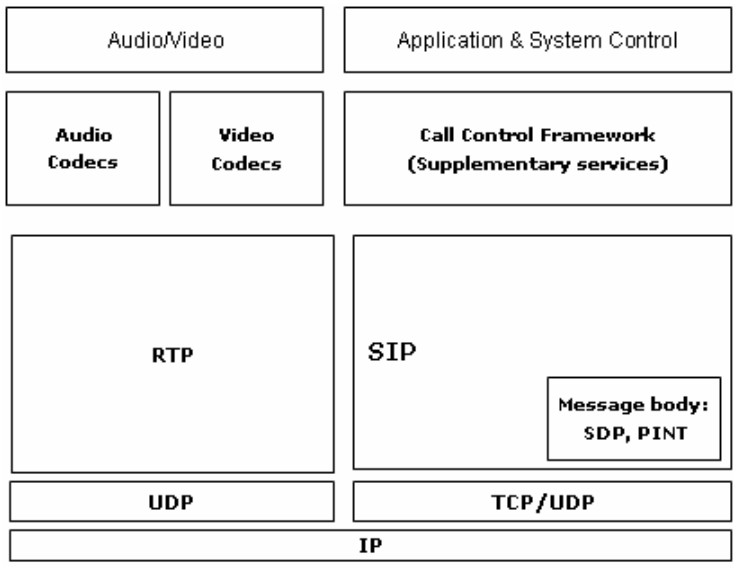
\includegraphics[width=3in]{images/sip_protocol_suite.png}
\end{center}

\subsection{Skype}
